%% ─── System: KB ──────────────────────────────────────────────────────────────
\section{KB: A Hybrid-Retrieval Codebase Knowledge System}
\label{sec:system}

\subsection{Knowledge Representation}

KB represents a codebase as three kinds of independently retrievable
\emph{units} stored in a SQLite database, rather than as a single graph of
atomic facts:
\begin{itemize}
  \item \textbf{Documents} --- whole markdown files (README, docs) stored
    verbatim in a \texttt{documents} table (\texttt{title}, \texttt{body},
    \texttt{content\_hash}, origin \texttt{git\_repo}); the retrieval unit is the
    entire document, not a sentence chunk.
  \item \textbf{Code symbols} --- exported declarations (functions, classes,
    interfaces, type aliases, constants) extracted by AST analysis and stored in
    a \texttt{code\_symbols} table with their name, \texttt{kind}, and source
    text.
  \item \textbf{Facts} --- curated natural-language claims in a \texttt{facts}
    table, retained for authoring provenance and as a third retrieval lane.
\end{itemize}

Each unit type has a paired FTS5 full-text index
(\texttt{documents\_fts}, \texttt{code\_symbols\_fts}, \texttt{facts\_fts}) and
an optional per-unit embedding vector (\texttt{doc\_embeddings},
\texttt{code\_embeddings}, and fact embeddings).  Documents and symbols are
associated through a flat \texttt{doc\_code\_links} table---a document is linked
to the symbols it describes.  This is deliberately \emph{not} a traversable
graph: there are no typed fact edges and no multi-hop neighborhoods.  An earlier
version of KB stored sentence-level facts in a \texttt{fact\_edges} graph and
walked it at query time; that graph was removed in favor of the flat,
depth-1 link table because unbounded neighborhood expansion made retrieval cost
scale with index connectivity rather than with the query.

\subsection{Indexing Pipeline}

\texttt{kb init} executes a fully deterministic indexing pipeline.
No LLM is invoked and no API cost is incurred.

\medskip
\noindent\textbf{Code symbols.}  For each source file, KB
invokes the \texttt{web-tree-sitter} WASM runtime with per-language export
queries to extract named declarations.  Each exported symbol becomes a
\texttt{code\_symbols} row keyed by \texttt{(git\_repo, rel\_path, name)}, storing
its kind and source text for later display and neural scoring.

\medskip
\noindent\textbf{Documents.}  Human-readable sources (README files, markdown
documentation) are ingested \emph{whole}: each file becomes one
\texttt{documents} row with a content hash for incremental re-indexing.  Open
Knowledge Format frontmatter is stripped so metadata never pollutes the body.
KB then records \texttt{doc\_code\_links} between a document and the symbols it
references.

\medskip
\noindent\textbf{Embeddings.}  After indexing completes, \texttt{kb init} runs a
best-effort embedding pass over documents and symbols: by default a local
on-device sentence-transformer (\texttt{all-MiniLM-L6-v2}); set
\texttt{KB\_EMBEDDER=gemini} to opt into hosted Gemini embeddings.  When no
embedder is available, rows keep a deterministic hash vector and neural scoring
degrades gracefully---init never blocks on embedding failure, and the lexical
lanes carry retrieval on their own.

The raylib snapshot in Table~\ref{tab:harvest-results}
(\RaylibKEntities{} entities, \RaylibKRels{} links)
completes init+scan in minutes on a laptop with no LLM indexing cost.

%% ─── Figure: KB Architecture (auto-rendered from figures/kb-arch.mmd) ─────────
\begin{figure}[t]
\centering
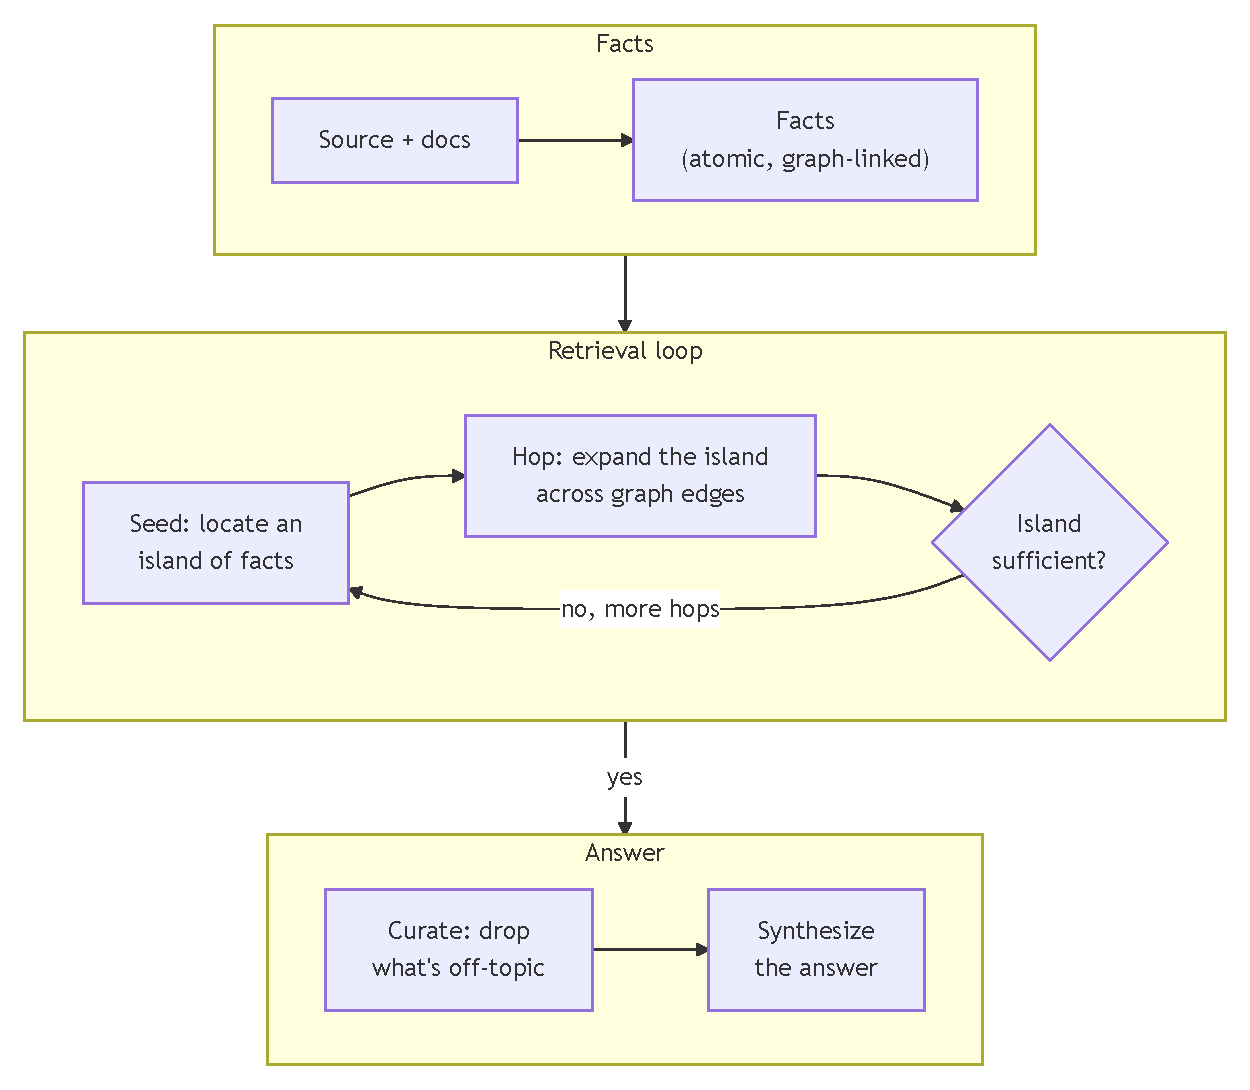
\includegraphics[width=\columnwidth]{figures/kb-arch.pdf}
\caption{KB indexing (top) feeds the hybrid retriever: six lexical/neural lanes over documents, symbols, and facts are fused by Reciprocal Rank Fusion, a depth-1 doc$\leftrightarrow$symbol hop enriches the pool, and a curator prunes before one-shot synthesis (bottom).}
\label{fig:kb-arch}
\end{figure}

\subsection{Retrieval: Hybrid Rank Fusion}
\label{subsec:retrieval}

At query time, KB runs a single-pass \emph{hybrid} retriever over the three unit
types.  For a query $q$ it opens six ranked lanes---each of
\{documents, code symbols, facts\} searched both lexically (BM25~\cite{robertson2009bm25}
over FTS5) and neurally (embedding cosine).  To avoid a full-table embedding scan
per query, the neural lanes re-rank the candidate pool that the lexical lanes
surfaced rather than scoring every vector in the index.

\medskip
\noindent\textbf{Reciprocal Rank Fusion.}  The six lists are combined with
Reciprocal Rank Fusion (RRF)~\cite{cormack2009rrf}: a unit at rank $i$ in a lane
contributes $1/(k + i)$ to its fused score, with damping $k = 60$.  RRF needs no
per-lane score calibration---it consumes only ranks---so lexical BM25 scores and
cosine similarities combine without a tuned weighting between them, and a unit
surfaced by several lanes accrues their contributions.

\medskip
\noindent\textbf{Depth-1 enrichment hop.}  After fusion, KB takes the top few
documents and symbols and follows \texttt{doc\_code\_links} exactly one hop: the
code a top document describes, and the documentation that describes a top symbol.
Hopped units enter \emph{below} every directly matched unit, so they enrich the
pool without displacing direct hits.  Because the link table is flat and the hop
is depth-1 by construction, retrieval cost is bounded by the candidate pool, not
by how densely the index is connected---the property the removed graph walk
lacked.  The top $\sim\!40$ fused units are handed to curation and synthesis.

\subsection{Post-Retrieval Curation}
\label{subsec:curation}

Rank fusion and the enrichment hop are deliberately \emph{broad}: they surface
units adjacent to, but not always directly about, the user's question.  When the
ranked pool is large enough, a \textbf{curator} runs \emph{before} synthesis.
It is judge-in-the-loop, not a static score floor:
\begin{enumerate}
  \item \textbf{Deterministic auto-keep}: units whose token overlap with the
    \emph{raw user question} exceeds a fixed threshold bypass the LLM (no cost,
    stable anchors).
  \item \textbf{Candidate cap}: only the top-ranked units enter the LLM verdict;
    the tail is dropped deterministically so large pools cannot overflow the
    structured keep/drop JSON.
  \item \textbf{Structured relevance verdict}: remaining candidates are sent to a
    single LLM call returning a structured verdict with \emph{keep} ids,
    \emph{gap} descriptions, and a \emph{sufficient} flag.
  \item \textbf{Drop}: every unit not in the keep set (except auto-kept rows) is
    removed from the synthesis context; there is no minimum keep fraction.
  \item \textbf{Gap re-discovery}: when the judge reports gaps and the set is not
    yet sufficient, the curator issues bounded hybrid searches per gap (excluding
    already-seen ids), merges new hits, and re-judges for up to a small round cap.
\end{enumerate}

On LLM or parse failure the curator \emph{fails safe} to the incoming pool for
small sets, and caps at the top-ranked subset for larger pools rather than
passing an unfiltered pool into synthesis.  Curator audit counts (kept, dropped,
re-queried) are recorded separately from the synthesis context for later
analysis---never injected back into the prompt as evidence.

\subsection{Answer synthesis}
\label{subsec:synthesis}

After retrieval and optional curation, \texttt{kb query} performs \emph{one-shot}
synthesis: a single LLM call over the curator-kept units (document bodies are
truncated to a per-unit character cap).  The synthesis prompt instructs
\emph{plain prose}: no inline ``(fact~$n$)'' citations and no trailing
Sources/Citations block; provenance is surfaced in a separate structured
evidence summary.  This is the path evaluated against the control agent in
\S\ref{subsec:results}---no multi-turn retrieval loop, matching how an external
agent would call KB for a standalone question.

%% ─── MOEL ─────────────────────────────────────────────────────────────────────
\section{MOEL: Multi-Objective Exploration Loss}
\label{sec:moel}

\subsection{Motivation}

Standard evaluation of LLM agents on code tasks measures whether the final
answer is correct.  This binary signal hides the cost of exploration: an agent
that issues 50 tool calls to reach a correct answer and one that issues 3 are
indistinguishable under pass/fail scoring.  Similarly, LLM-as-judge evaluators
have known failure modes (position bias, verbosity inflation, self-enhancement)
that inflate quality estimates when judges are not calibrated~\cite{zheng2023judging}.

MOEL addresses both problems by combining three normalized loss components into a
single scalar, evaluated under three controlled conditions per task.

\subsection{Three-Condition Evaluation Design}
\label{subsec:conditions}

The \emph{deep} MOEL evaluation runs each task under three toy-tool conditions
(Table~\ref{tab:moel-conditions}).  This differs from the \emph{harvest}
evaluation (\S\ref{sec:experiments}), where condition~N is a headless coding
agent with filesystem exploration tools and condition~K is \texttt{kb query}---the
pair that defines $\Delta S$.

\begin{table}[h]
\centering\small
\caption{Deep MOEL evaluation: toy-tool conditions per task (not the harvest N/K pair).}
\label{tab:moel-conditions}
\begin{tabular}{@{}p{1.6cm}p{3.4cm}p{1.6cm}@{}}
\toprule
\textbf{Cond.} & \textbf{Tools available} & \textbf{Purpose} \\
\midrule
\textbf{N} (raw FS) &
  {\footnotesize\texttt{read\_file}, \texttt{list\_directory},
  \texttt{search\_file\_contents}} &
  Worst-case baseline \\[3pt]
\textbf{K} (KB) &
  Full KB retrieval and action tools &
  Primary experiment \\[3pt]
\textbf{O} (Oracle) &
  Minimal facts injected in system prompt &
  Ceiling \\
\bottomrule
\end{tabular}
\end{table}

The primary hypothesis is $L_\text{MOEL}(N) > L_\text{MOEL}(K)$; secondary
goal is $L_\text{MOEL}(K) \approx L_\text{MOEL}(O)$ as the knowledge base
matures.  Harvest headline results (\S\ref{subsec:results}) use $\Delta S$ instead.

\subsection{Loss Functions}

\subsubsection*{$L_\text{jury}$ --- LLM Jury Semantic Loss}

$L_\text{jury}$ submits the candidate and reference to an ensemble of LLM
judges and aggregates their rubric scores.  Each judge assigns scores on
configurable rubric axes (correctness, usefulness, specificity, evidence
handling) on a 0--5 scale, and may optionally raise a \emph{veto flag}.

\medskip
\noindent\textbf{Bias mitigation.}  Four debiasing mechanisms are applied:
\begin{enumerate}
  \item \textbf{Verbosity normalization}: a $\log_{1+}$ length-scaling term is
    added to the rubric, penalizing unnecessary verbosity without penalizing
    accurate, detailed responses.
  \item \textbf{Position debiasing}: each judge evaluates both
    (candidate, reference) and (reference, candidate) orderings; the reported
    score is the average, and the absolute difference ($\Delta_\text{pos}$) is
    recorded as a consistency metric.
  \item \textbf{Self-enhancement down-weighting}: when a judge's model family
    matches the generator's, its weight is reduced to $0.5$.
  \item \textbf{Family diversity enforcement}: the ensemble must include
    $\geq 2$ judge families distinct from the generator family, preventing
    homogeneous scoring coalitions.
\end{enumerate}

\noindent\textbf{Minority-veto policy.}  If $\geq 2$ judges veto,
$L_\text{jury} = 1.0$; otherwise it equals $\bar{s}_w$, the weighted mean of
per-judge normalized scores:

\begin{equation}
L_\text{jury} = \begin{cases} 1.0 & \text{veto count} \geq 2 \\ \bar{s}_w & \text{otherwise} \end{cases}
\label{eq:ljury}
\end{equation}

\noindent\textbf{Statistical calibration.}  Jury scores are calibrated using
per-judge logistic regression:
\begin{equation}
P(\text{correct} \mid s) = \sigma(\beta_0 + \beta_1 s)
\label{eq:calibration}
\end{equation}
fitted on a 20-sample human-annotated dataset (10 pass / 10 fail, three human
judges per sample).  Generalization error is estimated via leave-one-out
cross-validation.  The pipeline is invoked once per judge model and stores
$(\beta_0, \beta_1)$ coefficients for use at scoring time.

\subsubsection*{$L_\text{trajectory}$ --- Trajectory Inefficiency Loss}

$L_\text{trajectory}$ penalizes two failure modes: taking more steps than a
configured ceiling, and repeating identical tool calls.  Let $H$ denote the
total step count, $h_\text{limit}$ the ceiling (default 20), and
$H_\text{dup}$ the number of duplicate (tool, args) pairs:

\begin{equation}
L_\text{traj} = \min\!\Bigl(
  \tfrac{1}{2}\min\!\bigl(\tfrac{H}{h_\text{lim}},1\bigr)
  + \tfrac{1}{2}\,\tfrac{H_\text{dup}}{H},\;1
\Bigr)
\label{eq:ltraj}
\end{equation}

Duplicate detection normalizes argument keys (alphabetical sort, whitespace
trim) so that logically identical calls with different JSON serializations are
correctly collapsed.

\subsubsection*{$L_\text{resource}$ --- Resource Consumption Loss}

$L_\text{resource}$ measures the weighted token footprint of a task run
against a configurable budget.  Following Anthropic's prompt caching pricing,
cached tokens are discounted by $\delta = 0.1$, and output tokens are weighted
at $\gamma = 1.0$:

\begin{equation}
L_\text{resource} = \min\!\left(
  \frac{C_\text{fresh} + \delta \cdot C_\text{cached} + \gamma \cdot C_\text{output}}
       {\text{budget}},\; 1
\right)
\label{eq:lresource}
\end{equation}

Token counts are drawn from per-step records that distinguish fresh, cached,
and output tokens; aggregated totals that lack this split are not used.

\subsection{MOEL Aggregation}

The three components combine into a single scalar:

\begin{equation}
L_\text{MOEL} = w_C \cdot L_\text{jury} + w_T \cdot L_\text{traj} + w_R \cdot L_\text{res}
\label{eq:lmoel}
\end{equation}

Default weights: $w_C = 0.5$, $w_T = 0.3$, $w_R = 0.2$.  The
constraint $w_C + w_T + w_R = 1$ is validated to within $10^{-6}$ and all
loss terms are bounded to $[0, 1]$.

\medskip
\noindent\textbf{Harvest adequacy scoring.}  The headline harvest evaluation
(\S\ref{subsec:success}) uses a complementary \emph{gain} formulation $S$ rather
than $L_\text{MOEL}$, but shares the same design principle: quality is measured
through an adequacy utility $\varphi_\tau$ (Eq.~\ref{eq:adequacy}) that treats
$\tau{=}3$ on the 0--4 rubric as ``good enough'' and applies diminishing
returns above it, so token and latency savings are not drowned out by marginal
rubric polish.

\subsection{Benchmark Alignment}

MOEL's three-condition design (N/K/O) mirrors SWE-ContextBench's context
injection conditions; $L_\text{resource}$ replicates that benchmark's
token-cost metric with the additional fresh/cached split.
CodeScaleBench's tool-validity tier corresponds to MOEL's condition comparison:
Condition N uses only primitive filesystem tools, Condition K adds the full KB
tool set.

